As mentioned in the precious section, errors can occur at every point in the
execution of an algorithm. State preparation, measurement, and gate operations
are examples of operations that are affected by these errors. Furthermore, the
errors occurring at any of these steps may propagate through the different
operations to the rest of the components of the system. This could lead to
cascading errors throughout the entire process, destroying all reliability in
the computation through loss of coherence. If a quantum computer is ever to be
realized, errors must be carefully contained.

It is in this context of error propagation that the concept of
\textit{fault-tolerant} quantum computing arises. A certain operation is said to
be fault-tolerant if a single error occurring at any step between two QEC cycles
causes at most one error at each of the logical blocks involved in the operation
\cite{Devitt_2013}. An example of fault-tolerant operation is shown in Fig.
\ref{fig:fault_tol} (b) where a bit-flip error in the top logical block
propagates only once to the bottom logical block (in contrast to (a) where it
propagates multiply). It is noteworthy that the constraint of only one
error propagating to different logical blocks can be relaxed when increasing the
code distance \cite{Devitt_2013}. In fact, for $d$ distance codes, it suffices
to require $d-2$ errors at each logical block.

\begin{figure}[htbp]
  \centering
  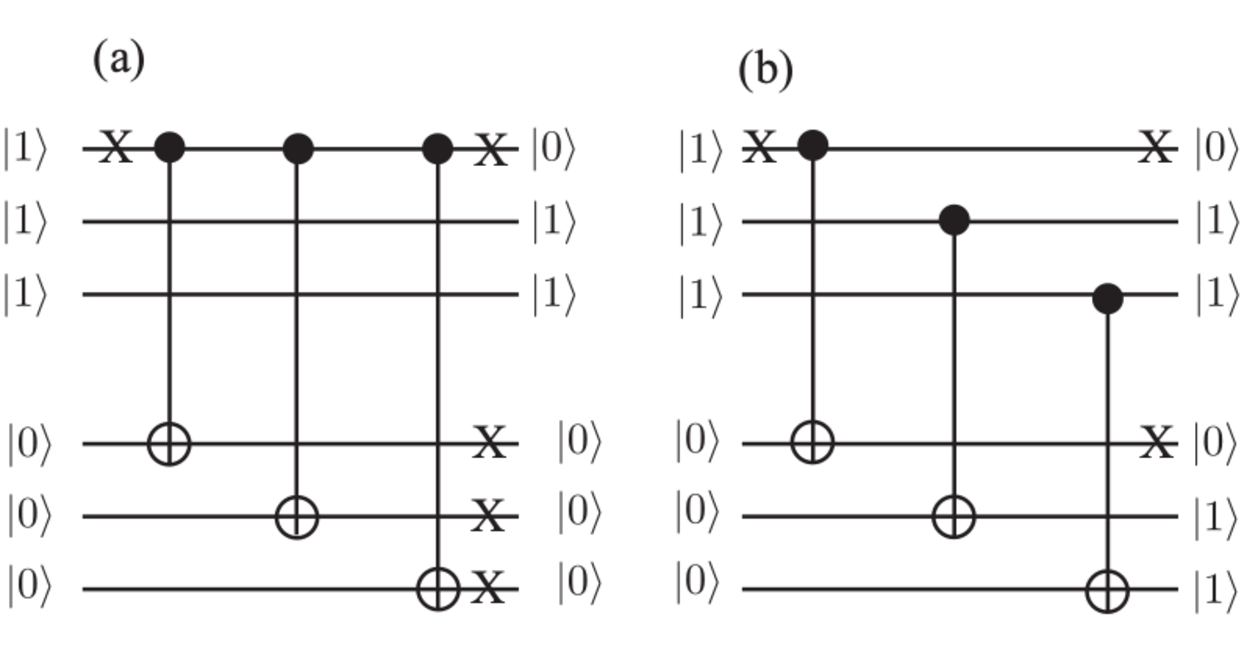
\includegraphics[width=0.5\textwidth]{images/fault_tolerance.pdf}
  \caption{Exmple of an operation that is not fault-tolerant (a) and one that is
    fault-tolerant (b). In these examples a bit-flip error in the top logical
    block propagates through the CNOT gates to the bottom logical block.}
  \label{fig:fault_tol}
\end{figure}

% Maybe logical error rates should be defined hered
However, it is not enough to have a fault tolerant set of operations in order to
implement a successful QEC protocol. Indeed, we want the logical error rate to
lower when increasing the code distance, either by means of concatenation or, in
the case of surface codes, by increasing the size of the surface. However, a high
error rate would prevent this from happening. In the case of surfaces codes, a
simple empirical equation that encapsulates the main properties of the logical
error rate obtained in simulations is
\cite{fowler12_surfac_codes}
\begin{equation}
  \label{eq:1}
  P_L = c\left(\frac{p}{p_{th}}\right)^{\frac{ d+1 }{2}},
\end{equation}
where d is the distance of the QEC protocol employed, $c$ is a constant that
depends on the exact characteristics of the error model, $p$ is the error rate
under sensible assumptions and $p_{th}$ is the error rate threshold. This
equation clearly shows the benefit of increasing the code distance, since for
$p<p_{th}$, the logical error rate decreases with increasing distance. Even
though these threshold error rates vary depending on the employed error model,
the current consensus puts the threshold at around $10^{-2}$ \cite{terhal15}
\cite{Versluis_2017}. However, it is yet to be shown experimentally a physical
system that accomplishes such low error rates.



%%% Local Variables:
%%% mode: latex
%%% TeX-master: "QEC_paper"
%%% End:
